\documentclass[aspectratio=169,10pt]{beamer}

\usetheme[numbering=fraction,progressbar=frametitle]{metropolis}

\usepackage[T1]{fontenc}
\usepackage[utf8]{inputenc}
\usepackage{booktabs}
\usepackage{graphicx}
\usepackage{pgfplots}
\usepackage{tikz}
\usepackage{listings}
\usepackage{xcolor}
\usepackage{tabularx}
\usepackage{array}

\pgfplotsset{compat=1.18,compat/show suggested version=false}
\graphicspath{{../results/plots/}}

\definecolor{DeckNavy}{HTML}{172033}
\definecolor{DeckTeal}{HTML}{0F766E}
\definecolor{DeckBlue}{HTML}{2563EB}
\definecolor{DeckGreen}{HTML}{15803D}
\definecolor{DeckAmber}{HTML}{B45309}
\definecolor{DeckRed}{HTML}{B91C1C}
\definecolor{DeckGray}{HTML}{64748B}

\setbeamercolor{normal text}{fg=DeckNavy,bg=white}
\setbeamercolor{frametitle}{fg=white,bg=DeckNavy}
\setbeamercolor{progress bar}{fg=DeckTeal,bg=DeckGray!25}
\setbeamercolor{alerted text}{fg=DeckAmber}
\setbeamercolor{block title}{fg=white,bg=DeckTeal}
\setbeamercolor{block body}{fg=DeckNavy,bg=DeckTeal!8}
\setbeamercolor{block title alerted}{fg=white,bg=DeckAmber}
\setbeamercolor{block body alerted}{fg=DeckNavy,bg=DeckAmber!10}
\setbeamercolor{block title example}{fg=white,bg=DeckGreen}
\setbeamercolor{block body example}{fg=DeckNavy,bg=DeckGreen!9}
\setbeamerfont{title}{size=\LARGE,series=\bfseries}
\setbeamerfont{subtitle}{size=\small}

\setbeamertemplate{itemize item}{\tikz\fill[DeckTeal] (0,0) circle (0.06);}
\setbeamertemplate{itemize subitem}{\tikz\fill[DeckBlue] (0,0) circle (0.045);}

\lstset{
  basicstyle=\ttfamily\scriptsize,
  keywordstyle=\color{DeckBlue}\bfseries,
  commentstyle=\color{DeckGray},
  stringstyle=\color{DeckGreen},
  breaklines=true,
  columns=fullflexible,
  keepspaces=true,
  showstringspaces=false
}

\newcommand{\metric}[3]{
  \begin{minipage}[t]{0.31\linewidth}
    {\Large\bfseries #1}\\[-1mm]
    {\footnotesize\color{DeckGray}#2}\\[-1mm]
    {\scriptsize\color{DeckTeal}#3}
  \end{minipage}
}

\newcommand{\runtimebox}[4]{
  \begin{tikzpicture}
    \node[
      draw=#1,
      rounded corners=2pt,
      line width=1pt,
      fill=#1!7,
      text width=0.88\linewidth,
      inner sep=5pt
    ] {
      {\bfseries #2}\\
      {\footnotesize #3}\\[1mm]
      {\scriptsize\color{DeckGray}#4}
    };
  \end{tikzpicture}
}

\title{WebAssembly Microservices\\with Spin/wasmtime vs OCI Containers}
\subtitle{Cold starts, isolation, throughput, and practical deployment guidance}
\author{Miłosz Słowiński \and Damian Staroń}
\date{Large Scale Computing 2026}

\begin{document}

\begin{frame}[plain]
  \vspace{12mm}
  {\LARGE\bfseries WebAssembly Microservices\\[1.5mm]with Spin/wasmtime vs OCI Containers}

  \vspace{5mm}
  {\large Cold starts, isolation, throughput, and practical deployment guidance}

  \vspace{8mm}
  \rule{0.8\linewidth}{0.5pt}

  \vspace{6mm}
  {\small Miłosz Słowiński \& Damian Staroń}\\
  {\small Large Scale Computing 2026}

  \vfill
  \begin{tabular}{lll}
    \textbf{44,471} movies & \textbf{1} shared Rust core & \textbf{2} runtime models
  \end{tabular}
\end{frame}

\begin{frame}{What we had to answer}
  \begin{block}{Assigned topic}
    Deploy a microservice application using Spin and wasmtime, then compare cold-start latency, memory isolation, and throughput against equivalent OCI containers.
  \end{block}

  \vspace{3mm}
  \begin{columns}[T,onlytextwidth]
    \begin{column}{0.48\linewidth}
      \textbf{The real question}
      \begin{itemize}
        \item Is Wasm practical as a serverless isolation substrate?
        \item What changes when the delivery unit is a WASI component instead of a container image?
        \item Which workloads actually benefit?
      \end{itemize}
    \end{column}
    \begin{column}{0.48\linewidth}
      \textbf{How we made it fair}
      \begin{itemize}
        \item Same application behavior before measuring speed.
        \item Same local machine and benchmark harness.
        \item Results interpreted by workload shape, not by technology hype.
      \end{itemize}
    \end{column}
  \end{columns}
\end{frame}

\begin{frame}[shrink=6]{Quick vocabulary}
  \begin{columns}[T,onlytextwidth]
    \begin{column}{0.48\linewidth}
      \runtimebox{DeckBlue}{WebAssembly}{Portable binary instruction format.}{Compiled Rust modules running outside the browser.}

      \vspace{1.8mm}
      \runtimebox{DeckGreen}{WASI}{System interfaces for Wasm.}{Controlled access to clocks, files, HTTP, randomness, and other host capabilities.}

      \vspace{1.8mm}
      \runtimebox{DeckTeal}{wasmtime}{Runtime for Wasm components.}{Executes WASI components and enforces the sandbox boundary.}
    \end{column}
    \begin{column}{0.48\linewidth}
      \runtimebox{DeckAmber}{Spin}{Framework and CLI for Wasm microservices.}{Provides HTTP triggers, local development, and deployment packaging.}

      \vspace{1.8mm}
      \runtimebox{DeckRed}{OCI / Docker}{Container image and runtime model.}{Packages native binaries plus OS-level dependencies into a standard deployable image.}
    \end{column}
  \end{columns}
\end{frame}

\begin{frame}{Two ways to deliver the same code}
  \begin{columns}[T,onlytextwidth]
    \begin{column}{0.48\linewidth}
      \begin{exampleblock}{Spin / WASI component}
        \begin{itemize}
          \item Application compiled to \texttt{wasm32-wasip2}.
          \item Host capabilities are explicit and narrow.
          \item Runtime boundary is the Wasm sandbox plus WASI.
          \item Good fit for request handlers, plugins, edge functions, and short-lived services.
        \end{itemize}
      \end{exampleblock}
    \end{column}
    \begin{column}{0.48\linewidth}
      \begin{alertblock}{OCI container}
        \begin{itemize}
          \item Application compiled as a native binary.
          \item Dependencies are packed into an image filesystem.
          \item Runtime boundary is process, namespace, cgroup, and container runtime isolation.
          \item Good fit for compatibility, native libraries, storage engines, and mature operations.
        \end{itemize}
      \end{alertblock}
    \end{column}
  \end{columns}
\end{frame}

\begin{frame}{What we built}
  \begin{center}
  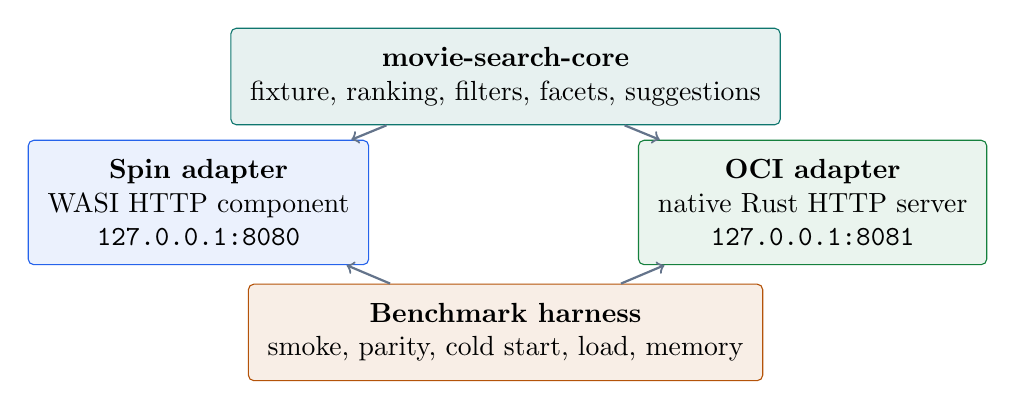
\begin{tikzpicture}[
    box/.style={draw, rounded corners=2pt, align=center, inner sep=7pt, minimum height=0.9cm},
    arrow/.style={->, thick, DeckGray}
  ]
    \node[box, fill=DeckTeal!10, draw=DeckTeal, minimum width=5.3cm] (core) at (0,1.4) {\textbf{movie-search-core}\\fixture, ranking, filters, facets, suggestions};
    \node[box, fill=DeckBlue!9, draw=DeckBlue, minimum width=3.8cm] (spin) at (-3.9,-0.2) {\textbf{Spin adapter}\\WASI HTTP component\\\texttt{127.0.0.1:8080}};
    \node[box, fill=DeckGreen!9, draw=DeckGreen, minimum width=3.8cm] (oci) at (3.9,-0.2) {\textbf{OCI adapter}\\native Rust HTTP server\\\texttt{127.0.0.1:8081}};
    \node[box, fill=DeckAmber!10, draw=DeckAmber, minimum width=5.4cm] (bench) at (0,-1.85) {\textbf{Benchmark harness}\\smoke, parity, cold start, load, memory};

    \draw[arrow] (core) -- (spin);
    \draw[arrow] (core) -- (oci);
    \draw[arrow] (bench) -- (spin);
    \draw[arrow] (bench) -- (oci);
  \end{tikzpicture}
  \end{center}

  \vspace{-1mm}
  \metric{44,471}{movie documents after deduplication}{same fixture}
  \hfill
  \metric{1 core}{shared Rust application logic}{same semantics}
  \hfill
  \metric{2 runtimes}{Spin/wasmtime and OCI}{same API}
\end{frame}

\begin{frame}[fragile]{Meilisearch-inspired demo features}
  \begin{columns}[T,onlytextwidth]
    \begin{column}{0.48\linewidth}
      \textbf{Added in the shared core}
      \begin{itemize}
        \item genre and year filters
        \item facets and year statistics
        \item deterministic sorting
        \item escaped highlights
        \item opt-in typo tolerance
        \item \texttt{/suggest} autocomplete
      \end{itemize}

      \begin{block}{Fairness rule}
        Legacy benchmark payloads stay unchanged. Enhanced features are opt-in and identical in both adapters.
      \end{block}
    \end{column}
    \begin{column}{0.49\linewidth}
      \begin{lstlisting}
{
  "q": "spce",
  "filter": {
    "genre": ["Science Fiction"],
    "year": {"gte": 1970}
  },
  "facets": ["genre", "year"],
  "highlight": ["title", "overview"],
  "typoTolerance": true
}
      \end{lstlisting}
    \end{column}
  \end{columns}
\end{frame}

\begin{frame}{Why not benchmark full Meilisearch?}
  \begin{block}{The initial idea was useful, but not fair enough}
    A direct ``Meilisearch in Docker vs Meilisearch in Spin'' comparison collapsed because the two sides could not share the same storage and ranking semantics.
  \end{block}

  \begin{columns}[T,onlytextwidth]
    \begin{column}{0.5\linewidth}
      \textbf{Blockers we found}
      \begin{itemize}
        \item Official Meilisearch uses LMDB and memory-mapped storage.
        \item Native dependencies such as crypto/runtime layers did not map cleanly to \texttt{wasm32-wasip2}.
        \item A custom Spin fallback would not be the same search engine.
      \end{itemize}
    \end{column}
    \begin{column}{0.46\linewidth}
      \textbf{Final decision}
      \begin{itemize}
        \item Keep Meilisearch as feasibility evidence.
        \item Build a deterministic service with one shared core.
        \item Compare the isolation models, not two different applications.
      \end{itemize}
    \end{column}
  \end{columns}
\end{frame}

\begin{frame}[fragile]{Shared API and parity checks}
  \begin{columns}[T,onlytextwidth]
    \begin{column}{0.46\linewidth}
      \textbf{Common endpoints}
      \begin{itemize}
        \item \texttt{GET /health}
        \item \texttt{GET /version}
        \item \texttt{GET /stats}
        \item \texttt{GET /movies?offset=\&limit=}
        \item \texttt{POST /search}
        \item \texttt{POST /suggest}
      \end{itemize}

      \vspace{1mm}
      \begin{lstlisting}[language=bash]
benchmarks/compare_results.sh
      \end{lstlisting}
    \end{column}
    \begin{column}{0.5\linewidth}
      \textbf{Parity queries}
      \begin{itemize}
        \item \texttt{space}
        \item \texttt{toy story}
        \item \texttt{dark knight}
        \item \texttt{romance}
        \item empty query
        \item enhanced filter/facet/highlight query
      \end{itemize}

      \vspace{1mm}
      \begin{block}{Acceptance rule}
        Both runtimes must return the same engine identity, document count, total hits, ordered \texttt{hit.id} values, facets, and suggestions.
      \end{block}
    \end{column}
  \end{columns}
\end{frame}

\begin{frame}{Benchmark methodology}
  \begin{columns}[T,onlytextwidth]
    \begin{column}{0.33\linewidth}
      \textbf{1. Correctness first}
      \begin{itemize}
        \item unit tests
        \item Spin build
        \item Docker build
        \item smoke and parity
      \end{itemize}
    \end{column}
    \begin{column}{0.33\linewidth}
      \textbf{2. Performance}
      \begin{itemize}
        \item 20 cold-start repeats
        \item load at concurrency 10, 50, 100, 200
        \item legacy and enhanced search payloads
        \item p50, p95, p99 latency
        \item response validation
      \end{itemize}
    \end{column}
    \begin{column}{0.33\linewidth}
      \textbf{3. Memory}
      \begin{itemize}
        \item idle samples
        \item under-load samples
        \item Docker stats for OCI
        \item host process RSS for Spin
      \end{itemize}
    \end{column}
  \end{columns}

  \vspace{4mm}
  \begin{block}{Important caveat}
    Memory accounting is operationally useful but not perfectly symmetric: Docker reports a container view, while Spin is measured as a host process tree.
  \end{block}
\end{frame}

\begin{frame}{Movie-search: cold start}
  \begin{columns}[T,onlytextwidth]
    \begin{column}{0.48\linewidth}
      \begin{table}
        \centering
        \small
        \begin{tabular}{llrr}
          \toprule
          Runtime & Path & Median & p95 \\
          \midrule
          OCI & \texttt{/health} & 21.1 ms & 38.7 ms \\
          Spin & \texttt{/health} & 145.6 ms & 202.7 ms \\
          OCI & first search & 431.8 ms & 854.8 ms \\
          Spin & first search & 370.0 ms & 446.3 ms \\
          \bottomrule
        \end{tabular}
      \end{table}

      \begin{block}{Interpretation}
        OCI reached a cheap readiness endpoint faster. Spin completed the recreated-service path through a real search request faster in this run.
      \end{block}
    \end{column}
    \begin{column}{0.5\linewidth}
      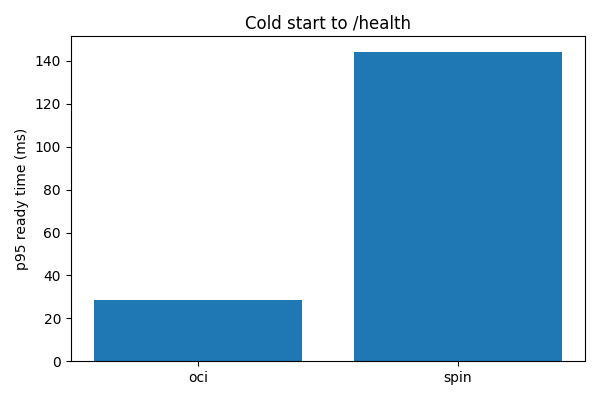
\includegraphics[width=\linewidth,height=0.68\textheight,keepaspectratio]{cold_start_p95.png}
    \end{column}
  \end{columns}
\end{frame}

\begin{frame}[shrink=5]{Movie-search: throughput and tail latency}
  \begin{columns}[T,onlytextwidth]
    \begin{column}{0.5\linewidth}
      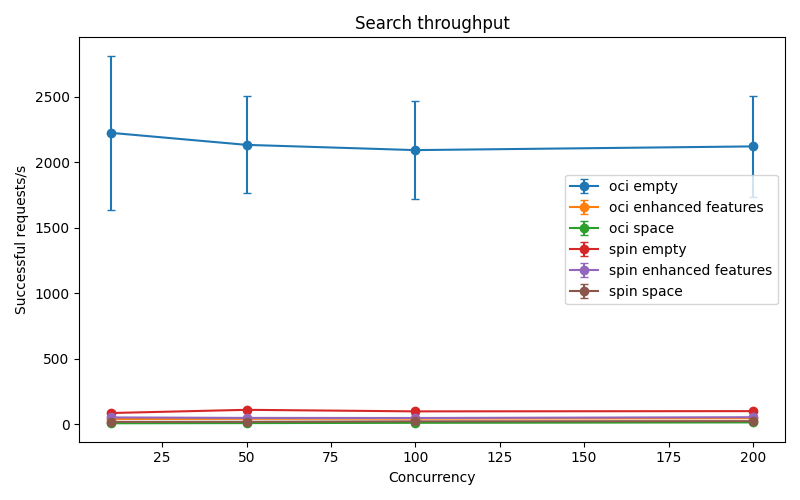
\includegraphics[width=\linewidth,height=0.58\textheight,keepaspectratio]{load_throughput.png}
    \end{column}
    \begin{column}{0.5\linewidth}
      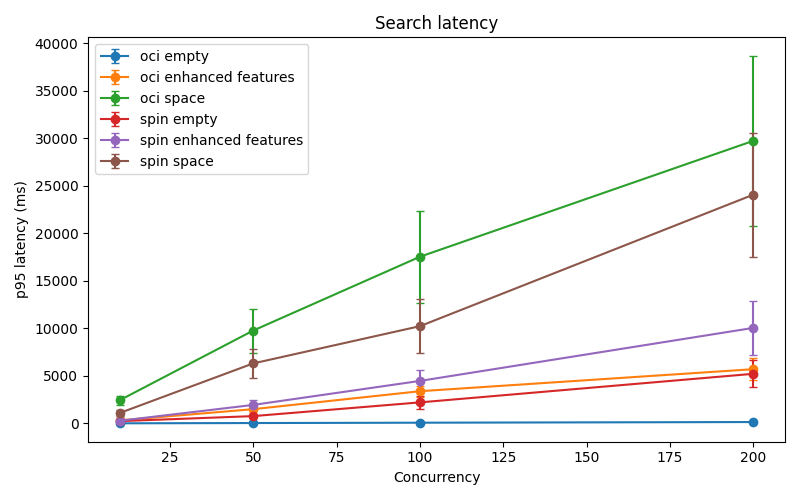
\includegraphics[width=\linewidth,height=0.58\textheight,keepaspectratio]{load_latency_p95.png}
    \end{column}
  \end{columns}

  \vspace{0.5mm}
  \scriptsize
  \begin{tabularx}{\linewidth}{>{\bfseries}lX}
    Empty query & OCI was much faster on the low-application-cost path: 2225 req/s vs 84 req/s at concurrency 10. \\
    \texttt{space} query & Spin had higher c=10 throughput, 16.8 req/s vs 6.0 req/s, with both runtimes timing out at c=200. \\
    Enhanced query & Spin led c=10 throughput, 50.8 req/s vs 38.7 req/s; tails grew quickly under high concurrency. \\
  \end{tabularx}
\end{frame}

\begin{frame}{Movie-search: memory is not automatically lower}
  \begin{columns}[T,onlytextwidth]
    \begin{column}{0.48\linewidth}
      \begin{table}
        \centering
        \small
        \begin{tabular}{llr}
          \toprule
          Runtime & Phase & Max observed \\
          \midrule
          OCI & idle & 34.6 MiB \\
          OCI & load & 37.4 MiB \\
          Spin & idle & 114.6 MiB \\
          Spin & load & 553.1 MiB \\
          \bottomrule
        \end{tabular}
      \end{table}

      \begin{alertblock}{Takeaway}
        Wasm gives a different isolation model. It does not guarantee lower RSS for every host, runtime, and workload.
      \end{alertblock}
    \end{column}
    \begin{column}{0.5\linewidth}
      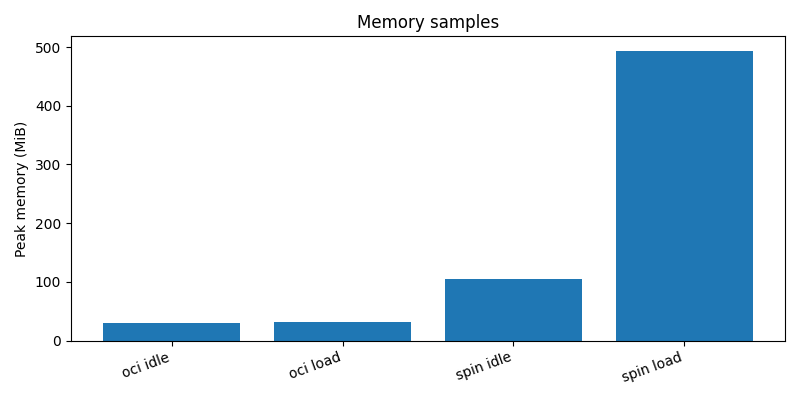
\includegraphics[width=\linewidth,height=0.68\textheight,keepaspectratio]{memory_peak.png}
    \end{column}
  \end{columns}
\end{frame}

\begin{frame}{Second workload: file-tools}
  \begin{columns}[T,onlytextwidth]
    \begin{column}{0.48\linewidth}
      \begin{exampleblock}{Spin implementation}
        \begin{itemize}
          \item \texttt{spin-file-tools-sdk4}
          \item Rust component with \texttt{spin-sdk = 4}
          \item Default port: \texttt{3000}
          \item Same request-level features as Docker side
        \end{itemize}
      \end{exampleblock}
    \end{column}
    \begin{column}{0.48\linewidth}
      \begin{alertblock}{Docker implementation}
        \begin{itemize}
          \item \texttt{docker-file-tools}
          \item Native Rust server with Axum
          \item Container port: \texttt{8081}
          \item Built as a Docker image
        \end{itemize}
      \end{alertblock}
    \end{column}
  \end{columns}

  \vspace{3mm}
  \begin{center}
    \small
    \texttt{/validate/json} \quad
    \texttt{/convert/json-to-csv} \quad
    \texttt{/convert/csv-to-json} \quad
    \texttt{/image/metadata} \quad
    \texttt{/image/grayscale} \quad
    \texttt{/image/resize}
  \end{center}
\end{frame}

\begin{frame}{File-tools: structure}
  \begin{center}
  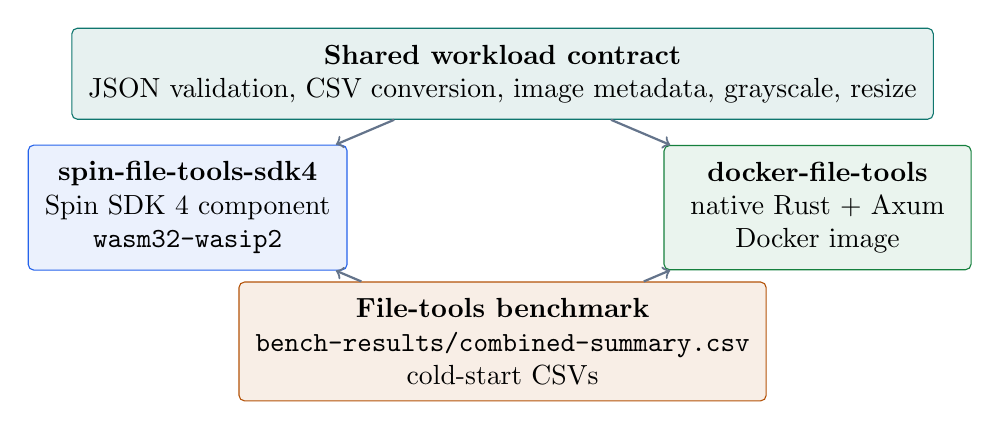
\begin{tikzpicture}[
    box/.style={draw, rounded corners=2pt, align=center, inner sep=6pt, minimum height=0.85cm},
    arrow/.style={->, thick, DeckGray}
  ]
    \node[box, fill=DeckTeal!10, draw=DeckTeal, minimum width=5.9cm] (contract) at (0,1.45) {\textbf{Shared workload contract}\\JSON validation, CSV conversion, image metadata, grayscale, resize};
    \node[box, fill=DeckBlue!9, draw=DeckBlue, minimum width=3.9cm] (spinft) at (-4.0,-0.25) {\textbf{spin-file-tools-sdk4}\\Spin SDK 4 component\\\texttt{wasm32-wasip2}};
    \node[box, fill=DeckGreen!9, draw=DeckGreen, minimum width=3.9cm] (dockerft) at (4.0,-0.25) {\textbf{docker-file-tools}\\native Rust + Axum\\Docker image};
    \node[box, fill=DeckAmber!10, draw=DeckAmber, minimum width=5.8cm] (benchft) at (0,-1.95) {\textbf{File-tools benchmark}\\\texttt{bench-results/combined-summary.csv}\\cold-start CSVs};

    \draw[arrow] (contract) -- (spinft);
    \draw[arrow] (contract) -- (dockerft);
    \draw[arrow] (benchft) -- (spinft);
    \draw[arrow] (benchft) -- (dockerft);
  \end{tikzpicture}
  \end{center}

  \vspace{-1mm}
  \metric{1 API shape}{same request classes}{not a toy hello-world}
  \hfill
  \metric{2 runtimes}{Spin SDK 4 and Docker}{same endpoints}
  \hfill
  \metric{2 workload types}{light JSON vs image-heavy}{different winners}
\end{frame}

\begin{frame}{File-tools: light request paths at concurrency 50}
  \begin{columns}[T,onlytextwidth]
    \begin{column}{0.63\linewidth}
      \begin{tikzpicture}
        \begin{axis}[
          width=\linewidth,
          height=0.62\textheight,
          ybar,
          bar width=8pt,
          ymin=0,
          ymax=3600,
          ylabel={requests / second},
          symbolic x coords={health,validate,json2csv,csv2json},
          xtick=data,
          xticklabel style={font=\scriptsize},
          legend style={at={(0.5,1.08)},anchor=south,legend columns=2,draw=none},
          grid=major,
          grid style={DeckGray!18}
        ]
          \addplot[fill=DeckGreen!70,draw=DeckGreen] coordinates {
            (health,1993) (validate,2309) (json2csv,2510) (csv2json,2417)
          };
          \addplot[fill=DeckTeal!70,draw=DeckTeal] coordinates {
            (health,3141) (validate,3112) (json2csv,2917) (csv2json,2914)
          };
          \legend{Docker,Spin}
        \end{axis}
      \end{tikzpicture}
    \end{column}
    \begin{column}{0.34\linewidth}
      \textbf{Result pattern}
      \begin{itemize}
        \item Spin was faster on these light paths.
        \item Throughput ratio ranged from 1.16x to 1.58x over Docker.
        \item p95 latency was similar or slightly better for Spin.
      \end{itemize}
    \end{column}
  \end{columns}
\end{frame}

\begin{frame}{File-tools: image-heavy paths at concurrency 50}
  \begin{columns}[T,onlytextwidth]
    \begin{column}{0.63\linewidth}
      \begin{tikzpicture}
        \begin{axis}[
          width=\linewidth,
          height=0.62\textheight,
          ybar,
          bar width=10pt,
          ymin=0,
          ymax=1600,
          ylabel={requests / second},
          symbolic x coords={metadata,grayscale,resize},
          xtick=data,
          xticklabel style={font=\scriptsize},
          legend style={at={(0.5,1.08)},anchor=south,legend columns=2,draw=none},
          grid=major,
          grid style={DeckGray!18}
        ]
          \addplot[fill=DeckGreen!70,draw=DeckGreen] coordinates {
            (metadata,1482) (grayscale,1014) (resize,594)
          };
          \addplot[fill=DeckTeal!70,draw=DeckTeal] coordinates {
            (metadata,591) (grayscale,239) (resize,84)
          };
          \legend{Docker,Spin}
        \end{axis}
      \end{tikzpicture}
    \end{column}
    \begin{column}{0.34\linewidth}
      \textbf{Result pattern}
      \begin{itemize}
        \item Docker was much faster for image processing.
        \item Resize at c=50: 594 req/s vs 84 req/s.
        \item Spin p95 resize latency reached about 799 ms.
      \end{itemize}
    \end{column}
  \end{columns}
\end{frame}

\begin{frame}{File-tools: cold start snapshot}
  \begin{columns}[T,onlytextwidth]
    \begin{column}{0.52\linewidth}
      \begin{tikzpicture}
        \begin{axis}[
          width=\linewidth,
          height=0.58\textheight,
          ybar,
          bar width=18pt,
          ymin=0,
          ymax=650,
          ylabel={median ms},
          symbolic x coords={Docker,Spin},
          xtick=data,
          nodes near coords,
          nodes near coords style={font=\scriptsize},
          grid=major,
          grid style={DeckGray!18}
        ]
          \addplot[fill=DeckGreen!70,draw=DeckGreen] coordinates {(Docker,296)};
          \addplot[fill=DeckTeal!70,draw=DeckTeal] coordinates {(Spin,559)};
        \end{axis}
      \end{tikzpicture}
    \end{column}
    \begin{column}{0.43\linewidth}
      \begin{table}
        \centering
        \small
        \begin{tabular}{lrrr}
          \toprule
          Runtime & n & Median & Range \\
          \midrule
          Docker & 5 & 296 ms & 264-497 \\
          Spin & 5 & 559 ms & 553-561 \\
          \bottomrule
        \end{tabular}
      \end{table}

      \begin{block}{How to read this}
        These file-tools cold-start samples are smaller than the main benchmark, so they support the practical story but do not replace the movie-search benchmark.
      \end{block}
    \end{column}
  \end{columns}
\end{frame}

\begin{frame}{What the two workloads taught us}
  \begin{columns}[T,onlytextwidth]
    \begin{column}{0.48\linewidth}
      \begin{exampleblock}{Spin/wasmtime looked attractive when}
        \begin{itemize}
          \item the handler was small and request-scoped;
          \item the workload stayed close to parsing, routing, and lightweight transformation;
          \item sandboxing and portability mattered more than native library reach;
          \item the deployment unit could be a capability-limited component.
        \end{itemize}
      \end{exampleblock}
    \end{column}
    \begin{column}{0.48\linewidth}
      \begin{alertblock}{OCI looked stronger when}
        \begin{itemize}
          \item native code paths and mature libraries dominated runtime cost;
          \item storage, memory mapping, or process tooling mattered;
          \item resource accounting had to match operations tooling;
          \item compatibility and ecosystem maturity were more important than minimal capability exposure.
        \end{itemize}
      \end{alertblock}
    \end{column}
  \end{columns}
\end{frame}

\begin{frame}{Recommendations}
  \begin{columns}[T,onlytextwidth]
    \begin{column}{0.32\linewidth}
      \textbf{Use Spin/Wasm for}
      \begin{itemize}
        \item edge/serverless handlers;
        \item plugin systems;
        \item untrusted extensions;
        \item small API adapters;
        \item capability-limited jobs.
      \end{itemize}
    \end{column}
    \begin{column}{0.32\linewidth}
      \textbf{Use OCI for}
      \begin{itemize}
        \item storage-heavy services;
        \item native databases;
        \item CPU-heavy media work;
        \item complex dependencies;
        \item standard production operations.
      \end{itemize}
    \end{column}
    \begin{column}{0.32\linewidth}
      \textbf{Always benchmark}
      \begin{itemize}
        \item cold path and warm path;
        \item low-cost and real endpoints;
        \item tail latency;
        \item memory from the same viewpoint where possible;
        \item correctness under load.
      \end{itemize}
    \end{column}
  \end{columns}
\end{frame}

\begin{frame}[fragile]{Demo path}
  \begin{columns}[T,onlytextwidth]
    \begin{column}{0.53\linewidth}
      \textbf{Movie-search}
      \begin{lstlisting}[language=bash]
cd spin-meili
spin build
spin up --listen 127.0.0.1:8080

cd oci-movie-search
docker compose up --build

benchmarks/compare_results.sh
      \end{lstlisting}
      \textbf{UI path:} search \texttt{space}, then enable enhanced mode and search \texttt{spce}.
    \end{column}
    \begin{column}{0.43\linewidth}
      \textbf{File-tools}
      \begin{lstlisting}[language=bash]
curl http://localhost:3000/routes
curl http://localhost:8081/routes

curl -X POST /validate/json
curl -X POST /image/resize
      \end{lstlisting}

      \begin{block}{Fallback}
        Show saved CSV files in \texttt{results/processed} and \texttt{bench-results}, then open the plots in \texttt{results/plots}.
      \end{block}
    \end{column}
  \end{columns}
\end{frame}

\begin{frame}{Final conclusions}
  \begin{columns}[T,onlytextwidth]
    \begin{column}{0.58\linewidth}
      \begin{itemize}
        \item We ran equivalent microservices in Spin/wasmtime and OCI with validated functional parity.
        \item The demo now includes search-product features, but they live in the same shared core.
        \item Wasm is practical for some serverless-style microservices, especially small isolated request handlers.
        \item OCI remains the safer default for native, storage-heavy, and operations-heavy services.
        \item ``Wasm is lighter than containers'' is too simple: workload shape and measurement viewpoint changed the result.
      \end{itemize}
    \end{column}
    \begin{column}{0.38\linewidth}
      \begin{block}{Bottom line}
        Choose the isolation substrate after measuring actual endpoint behavior.
      \end{block}

      \vspace{4mm}
      \textbf{Same code first.}\\
      \textbf{Measurements second.}\\
      \textbf{Recommendations last.}
    \end{column}
  \end{columns}
\end{frame}

\end{document}
